\documentclass[tikz]{standalone}
\usepackage{tikz}			% for drawing everything
	\usetikzlibrary{spy}	% for zooming
\usepackage{siunitx}		% for nice SI units
\usepackage{shadowtext}	% for shadowed text on the scalebar
	\shadowoffset{1pt}	% ideally the same as on line 13...
	\shadowcolor{green}	% ideally the same as on line 13...
\newcommand{\imsize}{\linewidth}% default width of image
\newlength\imagewidth% needed for correct scalebar
\newlength\imagescale% needed for correct scalebar
\begin{document}%
%----------
\tikzset{shadowed/.style={preaction={transform canvas={shift={(1pt,-1pt)}},draw=green, thick}}} % shadowed drawing https://tex.stackexchange.com/a/185853/828
\pgfmathsetlength{\imagewidth}{\imsize}%
\pgfmathsetlength{\imagescale}{\imagewidth/609}%
\def\x{376}% scalebar-x starting at golden ratio of image width of 609px = 376
\def\y{432}% scalebar-y at 90% of image height of 480px = 432
\def\mag{4}% magnification of inset
\def\size{75}% size of inset
\begin{tikzpicture}[x=\imagescale,y=-\imagescale,spy using outlines={rectangle,magnification=\mag,size=\size,connect spies}]
	\begin{scope}
		\clip (0,0) rectangle (609,480);
		%\clip (304.5,240.0) circle (240.0);
		\node[anchor=north west, inner sep=0pt, outer sep=0pt] at (0,0) {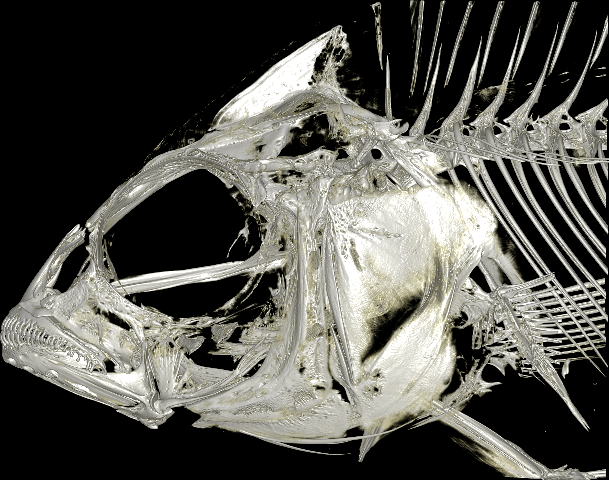
\includegraphics[width=\imagewidth]{head}};
	\end{scope}
	%\spy [red] on (309,180) in node at (0,0) [anchor=north west];
	% 475.587px = 18.486mm -> 100px = 3886.984um -> 12.863px = 500um, 2.573px = 100um
	\draw[|-|,blue,thick] (5,362) -- (340,25) node [sloped,midway,above,fill=white,semitransparent,text opacity=1] {\SI{18.486}{\milli\meter} (476px) TEMPORARY!};
	\draw[|-|,white,thick,shadowed] (\x,\y) -- (\x+128.63,\y) node [midway,above] {\shadowtext{\SI{5}{\milli\meter}}};
	%\draw[color=red, anchor=south west] (0,480) node [fill=white, semitransparent] {Legend} node {Legend};
\end{tikzpicture}%
%----------
\end{document}%
